\subsection{Provenance Data Model serialization}
There are two possible families of ProvenanceDM metadata serializations, examples for these can be found in the implementation section (\ref{sec:usecases-implementations}) and the links therein.
\begin{itemize}
 \item W3C serializations: PROV\-N, PROV\-JSON, PROV\-XML. These are serializations of the W3C provenance data model. They allow the possibility to add additional IVOA or ad hoc attributes to the basic ones in each class. This way the IVOA models can produce W3C compliant serializations.
% \item Mapping of ProvenanceDM classes onto tables with appropriate relationships. This can allow management by a TAP service (the model mapping is then described with the TAP schema). The serialization will result in a single table according to the query.

 %\TODO{TAP SCHEMA of the ProvenanceDM datamodel: Maybe Mathieu can provide us with a copy of the TAP schema he designed ?}

 \item Direct VOTABLE mapping by using some ad hoc mapping based on transcription of PROV-N format: this is called PROV-VOTABLE. Moreover in the future we could also define a VO-DML \citep{std:VODML} version of the mapping.
%The following is an example of provenance metadata in this PROV-VOTABLE format. Objects become tables, their classes are rendered by a utype. Attributes and relationships become FIELDS or PARAMS. The model attribute names also become VOTABLE utypes.  

\end{itemize}

This can be done using the voprov \footnote{\url{https://github.com/sanguillon/voprov}} python module.
The following is an example of a python program which describes the provenance and generates the different formats of serialization.
\begin{verbatim}
import sys
from prov.model import ProvDocument
from prov.dot import prov_to_dot
import pdb

try:
    provdoc = ProvDocument()
    provdoc.add_namespace('prov', 'http://www.w3.org/ns/prov#')
    provdoc.add_namespace('voprov', 'http://www.ivoa.net/documents/dm/provdm/voprov/')
    provdoc.add_namespace('ivo', 'http://www.ivoa.net/documents/rer/ivo/')
    provdoc.add_namespace('hips', 'http://cds.u-strasbg.fr/data/')

    provdoc.entity('ivo://CDS/P/DSS2color#RGB_NGC6946',\
        {'voprov:name':'RGB DSS2 image for NGC 6946', \
         'voprov:annotation':'This is a PNG RGB image built from DSS2 with Aladin for galaxy NGC 6946', \
         'voprov:doculink':'http://cds.u-strasbg.fr/aladin.gml'})

    provdoc.entity('ivo://CDS/P/DSS2/POSSII#POSSII.J-DSS2.143',\
        {'voprov:name':'POSSII Blue Survey DSS2 NGC6946', \
         'voprov:annotation':'This is the DSS2 digitazition of the Blue POSSII Schmidt survey around  NGC 6946', \
         'voprov:doculink':'http://cds.u-strasbg.fr/aladin.gm'})

    provdoc.entity('ivo://CDS/P/DSS2/POSSII#POSSII.F-DSS2.143',\
        {'voprov:name':'POSSII Red Survey DSS2 NGC6946', \
         'voprov:annotation':'This is the DSS2 digitazition of the Red POSSII Schmidt survey around NGC 6946', \
         'voprov:doculink':'http://cds.u-strasbg.fr/aladin.gml'})

    provdoc.entity('ivo://CDS/P/DSS2/POSSII#POSSII.N-DSS2.143',\
        {'voprov:name':'POSSII Infra Red Survey DSS2 NGC6946', \
         'voprov:annotation':'This is the DSS2 digitazition of the Infra red POSSII Schmidt survey around  NGC 6946', \
         'voprov:doculink':'http://cds.u-strasbg.fr/aladin.gm'})

    provdoc.activity('hips:AlaRGB1', '2017-04-18T17:28:00', '2017-04-19T17:29:00', \
          {'voprov:name':'Aladin RGB 1',\
           'voprov:annotation': 'Aladin RGB image generation for NGC 6946',\
           'voprov:desc_id': 'AlaRGB', \
           'voprov:desc_name': 'Aladin RGB image generation algorithm', \
           'voprov:desc_type': 'RGBencoding', \
           'voprov:desc_doculink':'http://cds.u-strasbg.fr/aladin.gml'})

    provdoc.used('hips:AlaRGB1', 'ivo://CDS/P/DSS2/POSSII#POSSII.J-DSS2.143')
    provdoc.used('hips:AlaRGB1', 'ivo://CDS/P/DSS2/POSSII#POSSII.F-DSS2.143')
    provdoc.used('hips:AlaRGB1', 'ivo://CDS/P/DSS2/POSSII#POSSII.J-DSS2.143')

    provdoc.wasGeneratedBy('ivo://CDS/P/DSS2color#RGB_NGC6946', 'hips:AlaRGB1', '')

    f_out = open('ex1.json','w')
    f_out.write(provdoc.serialize(indent=2))
    f_out.close()
    f_out = open('ex1.provn','w')
    f_out.write(provdoc.get_provn())
    f_out.close()
    provdoc.serialize(format='xml', destination='ex1.xml')
    f_out = open('ex1.votable','w')
    f_out.write(provdoc.serialize(format='votable',indent=2))
    f_out.close()

except Exception, e:
        print("Error while writing the file : %s !" %str(e))
        sys.exit(1)

\end{verbatim}

This is the PROV-N serialization:

\begin{verbatim}

document
  prefix ivo <http://www.ivoa.net/documents/rer/ivo/>
  prefix hips <http://cds.u-strasbg.fr/data/>
  prefix voprov <http://www.ivoa.net/documents/dm/provdm/voprov/>

  entity(ivo://CDS/P/DSS2color#RGB_NGC6946, [voprov:annotation="This is a PNG RGB image built from DSS2 with Aladin for galaxy NGC 6946", voprov:doculink="http://cds.u-strasbg.fr/aladin.gml", voprov:name="RGB DSS2 image for NGC 6946"])
  entity(ivo://CDS/P/DSS2/POSSII#POSSII.J-DSS2.143, [voprov:annotation="This is the DSS2 digitazition of the Blue POSSII Schmidt survey around  NGC 6946", voprov:doculink="http://cds.u-strasbg.fr/aladin.gm", voprov:name="POSSII Blue Survey DSS2 NGC6946"])
  entity(ivo://CDS/P/DSS2/POSSII#POSSII.F-DSS2.143, [voprov:annotation="This is the DSS2 digitazition of the Red POSSII Schmidt survey around NGC 6946", voprov:doculink="http://cds.u-strasbg.fr/aladin.gml", voprov:name="POSSII Red Survey DSS2 NGC6946"])
  entity(ivo://CDS/P/DSS2/POSSII#POSSII.N-DSS2.143, [voprov:annotation="This is the DSS2 digitazition of the Infra red POSSII Schmidt survey around  NGC 6946", voprov:doculink="http://cds.u-strasbg.fr/aladin.gm", voprov:name="POSSII Infra Red Survey DSS2 NGC6946"])
  activity(hips:AlaRGB1, 2017-04-18T17:28:00, 2017-04-19T17:29:00, [voprov:desc_id="AlaRGB", voprov:desc_type="RGBencoding", voprov:annotation="Aladin RGB image generation for NGC 6946", voprov:desc_name="Aladin RGB image generation algorithm", voprov:name="Aladin RGB 1", voprov:desc_doculink="http://cds.u-strasbg.fr/aladin.gml"])
  used(hips:AlaRGB1, ivo://CDS/P/DSS2/POSSII#POSSII.J-DSS2.143, -)
  used(hips:AlaRGB1, ivo://CDS/P/DSS2/POSSII#POSSII.F-DSS2.143, -)
  used(hips:AlaRGB1, ivo://CDS/P/DSS2/POSSII#POSSII.N-DSS2.143, -)
  wasGeneratedBy(ivo://CDS/P/DSS2color#RGB_NGC6946, hips:AlaRGB1, 2017-05-05T00:00:00)
endDocument

\end{verbatim}

This is the json serialization:

\begin{verbatim}

{
  "prefix": {
    "ivo": "http://www.ivoa.net/documents/rer/ivo/",
    "voprov": "http://www.ivoa.net/documents/dm/provdm/voprov/",
    "hips": "http://cds.u-strasbg.fr/data/"
  },
  "activity": {
    "hips:AlaRGB1": {
      "voprov:desc_doculink": "http://cds.u-strasbg.fr/aladin.gml",
      "voprov:desc_id": "AlaRGB",
      "prov:startTime": "2017-04-18T17:28:00",
      "voprov:annotation": "Aladin RGB image generation for NGC 6946",
      "voprov:desc_type": "RGBencoding",
      "voprov:desc_name": "Aladin RGB image generation algorithm",
      "prov:endTime": "2017-04-19T17:29:00",
      "voprov:name": "Aladin RGB 1"
    }
  },
  "wasGeneratedBy": {
    "_:id4": {
      "prov:time": "2017-05-05T00:00:00",
      "prov:entity": "ivo://CDS/P/DSS2color#RGB_NGC6946",
      "prov:activity": "hips:AlaRGB1"
    }
  },
  "used": {
    "_:id1": {
      "prov:entity": "ivo://CDS/P/DSS2/POSSII#POSSII.J-DSS2.143",
      "prov:activity": "hips:AlaRGB1"
    },
    "_:id3": {
      "prov:entity": "ivo://CDS/P/DSS2/POSSII#POSSII.N-DSS2.143",
      "prov:activity": "hips:AlaRGB1"
    },
    "_:id2": {
      "prov:entity": "ivo://CDS/P/DSS2/POSSII#POSSII.F-DSS2.143",
      "prov:activity": "hips:AlaRGB1"
    }
  },
  "entity": {
    "ivo://CDS/P/DSS2/POSSII#POSSII.J-DSS2.143": {
      "voprov:name": "POSSII Blue Survey DSS2 NGC6946",
      "voprov:annotation": "This is the DSS2 digitazition of the Blue POSSII Schmidt survey around  NGC 6946",
      "voprov:doculink": "http://cds.u-strasbg.fr/aladin.gm"
    },
    "ivo://CDS/P/DSS2/POSSII#POSSII.F-DSS2.143": {
      "voprov:name": "POSSII Red Survey DSS2 NGC6946",
      "voprov:annotation": "This is the DSS2 digitazition of the Red POSSII Schmidt survey around NGC 6946",
      "voprov:doculink": "http://cds.u-strasbg.fr/aladin.gml"
    },
    "ivo://CDS/P/DSS2/POSSII#POSSII.N-DSS2.143": {
      "voprov:name": "POSSII Infra Red Survey DSS2 NGC6946",
      "voprov:annotation": "This is the DSS2 digitazition of the Infra red POSSII Schmidt survey around  NGC 6946",
      "voprov:doculink": "http://cds.u-strasbg.fr/aladin.gm"
    },
    "ivo://CDS/P/DSS2color#RGB_NGC6946": {
      "voprov:name": "RGB DSS2 image for NGC 6946",
      "voprov:annotation": "This is a PNG RGB image built from DSS2 with Aladin for galaxy NGC 6946",
      "voprov:doculink": "http://cds.u-strasbg.fr/aladin.gml"
    }
  }
}

\end{verbatim}

This is the VOTABLE serialization:

\begin{verbatim}

<?xml version="1.0" encoding="UTF-8"?>
<VOTABLE version="1.2" xmlns="http://www.ivoa.net/xml/VOTable/v1.2" xmlns:hips="http://cds.u-strasbg.fr/data/" xmlns:ivo="http://www.ivoa.net/documents/rer/ivo/" xmlns:voprov="http://www.ivoa.net/documents/dm/provdm/voprov/" xmlns:xsi="http://www.w3.org/2001/XMLSchema-instance" xsi:schemaLocation="http://www.ivoa.net/xml/VOTable/v1.2 http://www.ivoa.net/xml/VOTable/VOTable-1.2.xsd">
  <RESOURCE type="provenance">
    <DESCRIPTION>Provenance VOTable</DESCRIPTION>
    <TABLE name="Usage" utype="voprov:used">
      <FIELD arraysize="*" datatype="char" name="activity" ucd="meta.id" utype="voprov:Usage.activity"/>
      <FIELD arraysize="*" datatype="char" name="entity" ucd="meta.id" utype="voprov:Usage.entity"/>
      <DATA>
        <TABLEDATA>
          <TR>
            <TD>hips:AlaRGB1</TD>
            <TD>ivo://CDS/P/DSS2/POSSII#POSSII.N-DSS2.143</TD>
          </TR>
        </TABLEDATA>
      </DATA>
    </TABLE>
    <TABLE name="Generation" utype="voprov:wasGeneratedBy">
      <FIELD arraysize="*" datatype="char" name="entity" ucd="meta.id" utype="voprov:Generation.entity"/>
      <FIELD arraysize="*" datatype="char" name="activity" ucd="meta.id" utype="voprov:Generation.activity"/>
      <DATA>
        <TABLEDATA>
          <TR>
            <TD>ivo://CDS/P/DSS2color#RGB_NGC6946</TD>
            <TD>hips:AlaRGB1</TD>
          </TR>
        </TABLEDATA>
      </DATA>
    </TABLE>
    <TABLE name="Activity" utype="voprov:Activity">
      <FIELD arraysize="*" datatype="char" name="id" ucd="meta.id" utype="voprov:Activity.id"/>
      <FIELD arraysize="*" datatype="char" name="name" ucd="meta.title" utype="voprov:Activity.name"/>
      <FIELD arraysize="*" datatype="char" name="start" ucd="" utype="voprov:Activity.startTime"/>
      <FIELD arraysize="*" datatype="char" name="stop" ucd="" utype="voprov:Activity.endTime"/>
      <FIELD arraysize="*" datatype="char" name="annotation" ucd="meta.description" utype="voprov:Activity.annotation"/>
      <FIELD arraysize="*" datatype="char" name="desc_id" ucd="" utype="voprov:ActivityDescription.id"/>
      <FIELD arraysize="*" datatype="char" name="desc_name" ucd="" utype="voprov:ActivityDescription.name"/>
      <FIELD arraysize="*" datatype="char" name="desc_type" ucd="meta.code.class" utype="voprov:ActivityDescription.type"/>
      <FIELD arraysize="*" datatype="char" name="desc_doculink" ucd="meta.ref.url" utype="voprov:ActivityDescription.doculink"/>
      <DATA>
        <TABLEDATA>
          <TR>
            <TD>hips:AlaRGB1</TD>
            <TD>Aladin RGB 1</TD>
            <TD>2017-04-18 17:28:00</TD>
            <TD>2017-04-19 17:29:00</TD>
            <TD>Aladin RGB image generation for NGC 6946</TD>
            <TD>AlaRGB</TD>
            <TD>Aladin RGB image generation algorithm</TD>
            <TD>RGBencoding</TD>
            <TD>http://cds.u-strasbg.fr/aladin.gml</TD>
          </TR>
        </TABLEDATA>
      </DATA>
    </TABLE>
    <TABLE name="Entity" utype="voprov:Entity">
      <FIELD arraysize="*" datatype="char" name="id" ucd="meta.id" utype="voprov:Entity.id"/>
      <FIELD arraysize="*" datatype="char" name="name" ucd="meta.title" utype="voprov:Entity.name"/>
      <FIELD arraysize="*" datatype="char" name="annotation" ucd="meta.description" utype="voprov:Entity.annotation"/>
      <DATA>
        <TABLEDATA>
          <TR>
            <TD>ivo://CDS/P/DSS2/POSSII#POSSII.J-DSS2.143</TD>
            <TD>POSSII Blue Survey DSS2 NGC6946</TD>
            <TD>This is the DSS2 digitazition of the Blue POSSII Schmidt survey around  NGC 6946</TD>
          </TR>
          <TR>
            <TD>ivo://CDS/P/DSS2/POSSII#POSSII.F-DSS2.143</TD>
            <TD>POSSII Red Survey DSS2 NGC6946</TD>
            <TD>This is the DSS2 digitazition of the Red POSSII Schmidt survey around NGC 6946</TD>
          </TR>
          <TR>
            <TD>ivo://CDS/P/DSS2/POSSII#POSSII.N-DSS2.143</TD>
            <TD>POSSII Infra Red Survey DSS2 NGC6946</TD>
            <TD>This is the DSS2 digitazition of the Infra red POSSII Schmidt survey around  NGC 6946</TD>
          </TR>
          <TR>
            <TD>ivo://CDS/P/DSS2color#RGB_NGC6946</TD>
            <TD>RGB DSS2 image for NGC 6946</TD>
            <TD>This is a PNG RGB image built from DSS2 with Aladin for galaxy NGC 6946</TD>
          </TR>
        </TABLEDATA>
      </DATA>
    </TABLE>
    <INFO name="QUERY_STATUS" value="OK"/>
  </RESOURCE>
</VOTABLE>

\end{verbatim}
  
Such serializations can be retrieved through Access protocols (see \ref{AccessPro} ) or directly integrated in datasets headers or "associated metadata" in order to provide provenance metadata for these datasets. 

\subsection{Graphical formats}
\label{Graphics}
The voprov python module can also provide provenance information in graphical formats: PNG, SVG and PDF.
In the above example, you have to add the following instructions in your python program:

\begin{verbatim}
    dot = prov_to_dot(provdoc, use_labels=True)
    dot.write_png('ex1.png')
    dot.write_svg('ex1.svg')
    dot.write_pdf('ex1.pdf')
\end{verbatim}

\begin{figure}
\centering
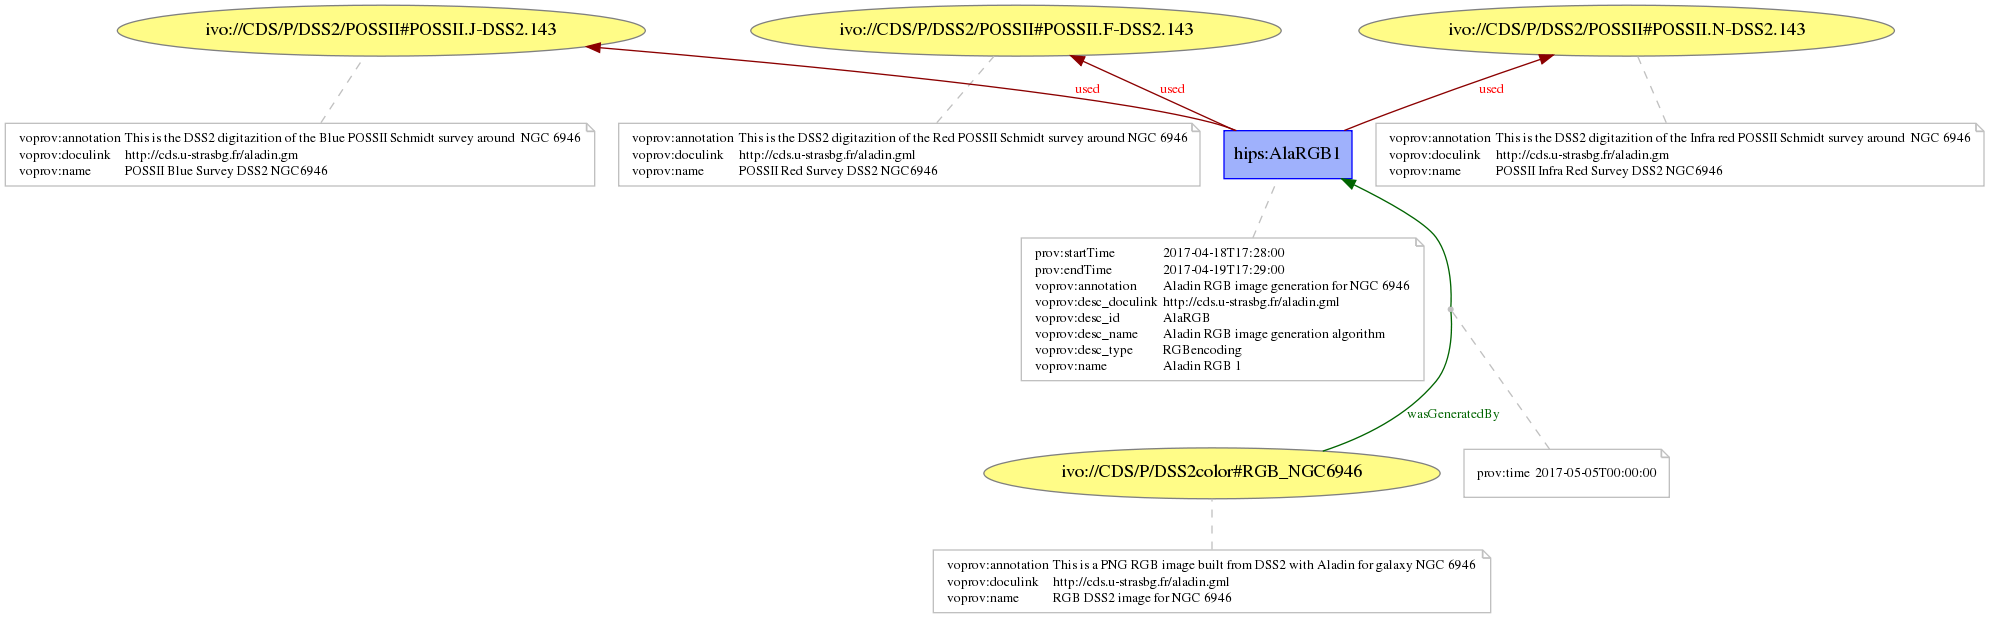
\includegraphics[width=0.9\textwidth]{access_ex1.png}
\caption{Example: png format@}
\label{fig:example}
\end{figure}


\subsection{Access protocols}
\label{AccessPro}
We envision two possible access protocols:
\begin{itemize}
\item ProvDAL: retrieve provenance information based on given id of a data entity or activity

ProvDAL is a service the interface of which is organized around one main PARAMETER, the ``ID'' of the entity (obs\_publisher\_did of an ObSDataSet for example). The response is given in one of the following formats: PROV-N, PROV-JSON, PROV-XML, PROV-VOTABLE. Additional parameters can complete ID to refine the query. FORMAT allows to choose the output format. STEP allows to discriminate between STEP=LAST which gives the last step in the provenance chain and STEP=ALL which gives the whole chain.
Multiple ID PARAMETER is allowed in order to retrieve several data set provenance details at the same time.
\item ProvTAP: allows detailed queries for provenance information, discovery of datasets based on 
e.g. code version.

ProvTAP is a TAP service implementing the ProvenanceDM data model. The data model mapping is included in the TAP schema. The mapping of ProvenanceDM classes and attributes onto tables and colomns of the schema with the appropriate relationships, datatypes, units, utypes and ucds is done similarly to the PROV-VOTABLE serialization. The query response will result in a single table according to the query.
 This  single table is joining information coming from one or several ``provenance'' tables available in the database. 

A special case is considered where ProvenanceDM and ObsCore are both implemented in the same TAP service and queried together. The TAP response is then providing an Obscore table with a ProvenanceDM extension. We can imagine that in the future this could be hard-coded and registered as an ObsTapProv service. 


\item Do we need combined query possibilities, i.e. ask for ObsCore-fields and Provenance fields
in one query? Or rather use a 2-step-process, decoupling them from each other?
\end{itemize}


%\TODO{Also look at PROV-AQ from the W3C.}
